\section{Описание}
Нужно построить график распределения терминов в полученном корпусе по частотностям в логарифмической шкале и наложить на него график закона Ципфа.

\vspace{2em}
\noindent\textbf{Закон Ципфа.} Закон Ципфа --- эмпирический закон, описывающий распределение. Он утверждает, что если все слова некоторого корпуса упорядочить по убыванию частоты их использования, то частота $f_r$ $r$-го по популярности слова будет приблизительно обратно пропорциональна его рангу $r$.
\\ \\
Математически закон записывается как:
\[
f_r \approx \frac{C}{r^{\alpha}},
\]
где:
\begin{itemize}
    \item $f_r$ --- частота слова, имеющего ранг $r$,
    \item $r$ --- ранг слова (1 для самого частого, 2 для следующего и т.д.),
    \item $C$ --- константа, часто близкая к частоте самого распространенного слова,
    \item $\alpha$ --- параметр, близкий к 1 для естественных языков (классический закон Ципфа).
\end{itemize}


В логарифмической шкале зависимость становится линейной:
\[
\log(f_r) \approx \log(C) - \alpha \cdot \log(r).
\]
Таким образом, на графике в двойных логарифмических координатах ($\log r$ по оси X, $\log f_r$ по оси Y) эмпирические данные, подчиняющиеся закону Ципфа, должны лечь приблизительно на прямую линию с отрицательным наклоном $-\alpha$.

\vspace{2em}
\noindent\textbf{Назначение и применение.}
Анализ распределения слов по закону Ципфа используется для:
\begin{itemize}
    \item Исследования статистических свойств языка и текстовых корпусов
    \item Верификации качества построения корпуса (естественные тексты обычно следуют этой закономерности).
    \item Выявления особенностей стиля или предметной области по отклонениям от классического распределения
    \item Оптимизации в информационном поиске и лингвистике (сжатие данных, построение словарей)
\end{itemize}

\pagebreak

\section{Исходный код}

Для построения графика по закону Ципфа был написан скрипт на Python.

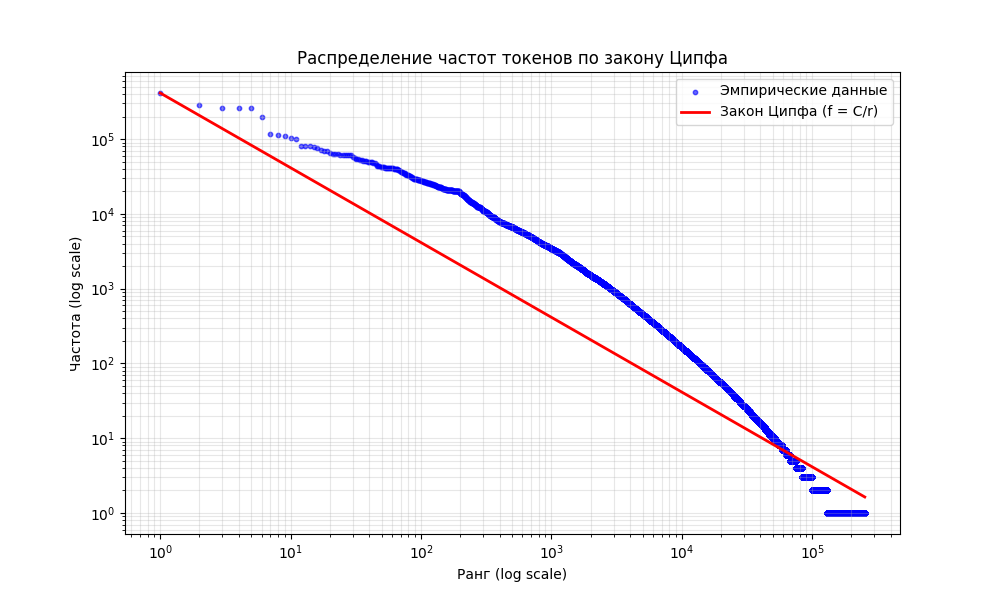
\includegraphics[width=\textwidth, height=\textheight, keepaspectratio]{pics/Zipf.png}

В результате видим, что частотность слов в нашем корпусе (22.2 млн токенов) подчиняется степенному закону, то етсть вероятность слова примерно обратно пропорциональна его рангу. Отклонения от идеальной прямой в области высоких рангов (редкие слова) характерны для реальных данных и могут быть связаны с ограниченным объемом выборки.

\begin{lstlisting}[language=Python]
# =========================
# ...
    for filename in sorted(os.listdir(dir_path)):
        if filename.endswith(".txt"):
            file_path = os.path.join(dir_path, filename)
            try:
                with open(file_path, 'r', encoding='utf-8') as f:
                    content = f.read().strip()
                    if content:
                        tokens = content.split()
                        all_tokens_counter.update(tokens)
            except Exception as e:
                print(f"Ошибка при чтении файла {filename}: {e}")
# ...
# =========================
    
    sorted_frequencies = sorted(all_tokens_counter.values(), reverse=True)
    
    ranks = list(range(1, len(sorted_frequencies) + 1))
    frequencies = sorted_frequencies
    
    C = frequencies[0]
    zipf_frequencies = [C / r for r in ranks]
    
    plt.figure(figsize=(10, 6))
    
    plt.scatter(ranks, frequencies, s=10, alpha=0.6, label='данные', color='blue')
    
    plt.plot(ranks, zipf_frequencies, 'r-', linewidth=2, label='Ципф (f = C/r)')
    
    plt.xscale('log')
    plt.yscale('log')
    plt.xlabel('Ранг (log scale)')
    plt.ylabel('Частота (log scale)')
    plt.grid(True, which="both", ls="-", alpha=0.3)
    plt.legend()
# ...
# =========================
    
\end{lstlisting}

\pagebreak

